% Chapter 3

\chapter{General Polynomial-Chaos}
Die hier aufgezeigte Einführung in das general Polynomial-Chaos (gPC) ist angelehnt an Xiu in \autocite{dongbinxiu2010}.
\section{Approximation von Zufallsvariablen}
Anhand des Beispiels \ref{bsp:hermitechaos} des Hermite-Chaos haben wir bereits gesehen, dass für gewisse Orthonormalbasen von Polynomen $\lbrace H_i\rbrace$ und Zufallsvariablen $Y$ mit passenden stochastischen Verteilungen die Beziehung
\[\langle H_i(x),H_j(x)\rangle_{L_w^2(S)} =\E_Y \left[H_i(Y)H_j(Y)\right]=\delta_{ij}\]
erfüllt wird. Ein feiner Unterschied ist dabei, dass die Polynome einmal mit reellem Argument und einmal mit der Zufallsvariable $Y$ als Argument aufgefasst werden.
\begin{mathdef}[General Polynomial-Chaos Basis]
\label{def:gpc}
Sei $Y$ eine reelle Zufallsvariable mit Verteilungsfunktion $F_Y(y)=P(Y\le y)$ und endlichen Momenten
\[\E\left[|Y|^{2\ell}\right]=\int |y|^{2\ell}dF_Y(y)<\infty,\quad \ell\in \N_0\]
Existieren Polynome $\Phi_i\in\Poly_i$, insbesondere $\Phi_0\equiv const$, welche die Bedingung
\begin{equation}
\label{eqn:gpc_basicortho}
\E\left[\Phi_i(Y)\Phi_j(Y)\right]=\delta_{ij},\quad i,j\in\N_0
\end{equation}
erfüllen, so nennt man diese \emph{general Polynomial-Chaos Basis-Funktionen}.\\
Ist $Y$ stetig, so existiert eine Dichtefunktion $\rho>0$, so dass $dF_Y(y)=\rho(y)dy$ auf $I$. In diesem Fall lässt sich die Bedingung (\ref{eqn:gpc_basicortho}) schreiben als
\begin{equation}
\label{eqn:gpc_ortho}
\E\left[\Phi_i(Y)\Phi_j(Y)\right]=\int_I \Phi_i(y)\Phi_j(y)\rho(y)dy=\delta_{ij},\quad i,j\in\N_0
\end{equation}
\end{mathdef}
\begin{mathbem}
Betrachten wir die Orthogonalitätsbedingung (\ref{eqn:gpc_ortho}), so wird klar, dass diese direkt der Orthogonalität des Raumes $L_\rho^2(I)$ entspricht. Die Polynome erfüllen somit nach Satz \ref{threetermexist} eine Drei-Term-Rekursion und bilden eine Orthonormalbasis bezüglich $L_\rho^2(I)$.\\
Man beachte, dass die hier vorgenommene Normierung der Basis keine Beschränkung der Allgemeinheit darstellt. Gilt als Bedingung nur
\[\langle H_i,H_j\rangle_{L_w^2(S)} =\E_Y \left[H_i(Y)H_j(Y)\right]=\gamma_i\delta_{ij},\quad i,j\in\N_0,\gamma_i>0\]
so müssen die Polynome $H_i$ lediglich durch die Normalisierungskonstanten $\sqrt{\gamma_i}=\sqrt{\E\left[\Phi_i^2(Y)\right]}$ geteilt werden.\\
Ist $Y$ keine stetige sondern eine diskrete Zufallsvariable, so ändert sich die Notation und aus obigen Integralen würden Reihen, die Kernaussagen blieben aber dieselben. Wir werden jedoch im Folgenden stets stetige Zufallsvariablen verwenden.
\end{mathbem}
Eine Übersicht von einigen bekannten Verteilungen und Polynombasen ist in Tabelle \ref{table:chaos} gegeben. Details zu stetigen Verteilungen finden sich im Anhang \ref{AppendixA}.\\
\begin{table}
\centering
\begin{tabular}{c|ccc}
 & Verteilung von $Y$ & gPC-Basispolynome & Träger \\ 
\hline 
Stetig & Normal & Hermite & $(-\infty,\infty)$ \\ 
 & Gamma & Laguerre & $[0,\infty)$ \\ 
 & Beta & Jacobi & $[-1,1]$ \\
 & Gleich & Legendre & $[-1,1]$ \\  
\hline 
Diskret & Poisson & Charlier & $\lbrace 0,1,2,\dots\rbrace$ \\ 
 & Binomial & Krawtchouk & $\lbrace 0,1,\dots,E\rbrace$ \\ 
 & Negativ Binomial & Meixner & $\lbrace 0,1,2,\dots\rbrace$ \\  
 & Hypergeometrisch & Hahn & $\lbrace 0,1,\dots,E\rbrace$
\end{tabular}
\caption{gPC-Beziehung zwischen orthogonalen Polynombasen und stochastischen Verteilungen. $E\in\N_0$ ist dabei ein beliebiger Parameter für gewisse diskrete Verteilungen.}
\label{table:chaos}
\end{table}

Das Ziel ist nun, mithilfe einer gPC-Orthonormalbasis eine Funktion $f(Y)$ einer Zufallsvariablen $Y$ zu approximieren. Wir wollen nun einen Einblick dazu bekommen, was an dieser Stelle mit "`approximieren"' gemeint ist.
\begin{mathdef}[Starke gPC-Konvergenz]
Sei $f(Y)$ eine Funktion einer Zufallsvariablen $Y$ mit Dichte $\rho_Y$ und Träger $I_Y$. Eine general Polynomial-Chaos Approximation $f_M(Y)\in\Poly_M(Y)$ konvergiert in einem starken Sinne gegen $f(Y)$, wenn \[\norm{f(Y)-f_M(Y)}_{L_{\rho_Y}^2(I_Y)}\to 0\text{ für }{M\to\infty}\]
\end{mathdef}
Die starke gPC-Konvergenz entspricht also direkt der in Kapitel \ref{sec:poly_approx} vorgestellten spektralen Konvergenz, entsprechend ist die Konvergenzordnung abhängig von der Glattheit der Funktion $f$. Ohne Beweis folgt aus der starken gPC-Konvergenz auch die Konvergenz in Wahrscheinlichkeit und schlussendlich die Konvergenz in Verteilung.
\begin{mathbem}
Ist die Funktion $f$ oder ihre Abhängigkeit von der Zufallsvariablen $Y$ nicht konkret bekannt, sondern liegt diese beispielsweise nur als Verteilungsfunktion vor, so ist es dennoch möglich eine gPC-Approximation in einem schwachen Sinne zu erhalten. Für Details sei auf \autocite[Kapitel 5.1.2]{dongbinxiu2010} verwiesen.\\
Ein illustratives Beispiel ist in Abbildung \ref{fig:gpcweakconv} gegeben. Dort verwenden wir die Bestapproximation bezüglich $L_\rho^2(-\infty,\infty)$, wobei $\rho$ die Dichtefunktion der Normalverteilung ist, die Orthonormalbasis aus den Hermite-Polynomen $H_m$ besteht und $Y$ eine normalverteilte Zufallsvariable ist. Es ist
\[f_M(Y)=\sum_{m=0}^M\hat{f}_mH_m(Y), \quad \hat{f}_m=\E[f(Y)H_m(Y)]\]
die Bestapproximation an die Funktion $f(Y)$ in $\Poly_M(Y)$. Wir nehmen an, dass wir nur die Verteilung von $Z=f(Y)$ kennen und $Z\sim\text{Beta}(0.2,3.)$ in $[-1,1]$.\\
Dann tritt bei der Berechnung von $\E[ZH_m(Y)]$ eine Schwierigkeit auf: Es ist in dieser Form nicht möglich den Erwartungswert zu berechnen, da die Zufallsvariablen $Z$ und $H_m(Y)$ zu verschiedenen Wahrscheinlichkeitsräumen gehören. Hierzu ist es nun hilfreich, mithilfe der Inversionsmethode die beiden Verteilungen auf einen gemeinsamen Wahrscheinlichkeitsraum $\mathcal{U}(0,1)$ zu "`normieren"'. Dann gilt
\[\hat{f}_m=\E_U\left[F_Z^{-1}(U)H_m(F_Y^{-1}(U))\right]=\int_0^1F_Z^{-1}(u)H_m(F_Y^{-1}(u))du\]
und $f_M(Y)$ konvergiert in Verteilung gegen $f(Y)$ für $M\to\infty$.
\begin{figure}[!htb]
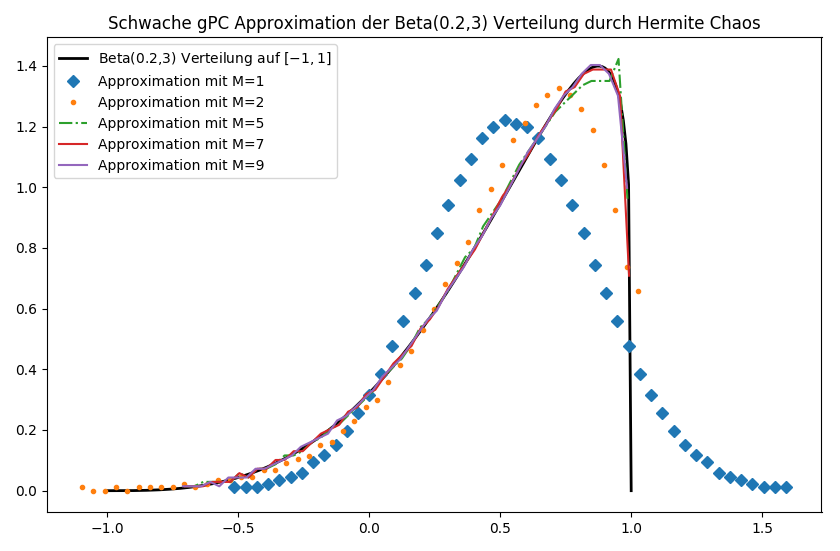
\includegraphics[width=\textwidth]{Figures/gpc_weak_convergence.png}
\caption{Schwache Konvergenz von Hermite gPC-Approximation zu einer $\text{Beta}(0.2,3.)$ verteilten Zufallsvariablen. Dargestellt sind Approximationen an die Dichtefunktionen, welche über Histogramme von 50 gleich großen Intervallen angenähert werden.}
\label{fig:gpcweakconv}
\end{figure}
\end{mathbem}

\section{Mehrdimensionale Zufallsräume}
Wie bereits diskutiert, sei der Zufallsraum durch einen Zufallsvektor $Y=(Y_1,\dots,Y_N)^T$ mit stochastisch unabhängigen Komponenten $Y_i$ mit bekannter Verteilung vollständig parametrisiert. Als mehrdimensionale Erweiterung von Definition \ref{def:gpc} führen wir an dieser Stelle das multivariate gPC-ein.
\begin{mathdef}[Multivariate gPC]
Sei $P\in\N_0$ der fest gewählte maximale Polynomgrad. Sei weiter $Y=(Y_1,\dots,Y_N)^T$ ein Zufallsvektor, dessen unabhängige Komponenten $Y_k$ eine gPC-Basis $\lbrace \Phi_i^{(k)}\in\Poly_P(Y_k)\mid i=0,\dots,P\rbrace$ besitzen. Ist $m=(m_1,\dots,m_N)\in\N_0^N$ ein Multi-Index mit $|m|=m_1+\dots+m_N$, so sind die $N$-variate gPC-Basis-Funktionen vom Grad $P$ definiert als 
\[\Phi_m(Y)=\Phi_{m_1}(Y_1)\cdot\ldots\cdot\Phi_{m_N}(Y_N),\quad 0\le |m|\le P\]
\end{mathdef}

\begin{mathbem}
Der von den multivariate gPC-Funktionen aufgespannte Raum $\Poly_P^N$ ist der Raum aller Polynome vom Grad höchstens $P$ in $N$ Variablen
\[\Poly_P^N(Y)\coloneqq \left\lbrace p\colon I_Y\to \R \mid p(Y)=\sum_{|m|\le P}c_m\Phi_m(Y)\right\rbrace\]
Die Dimension des Raumes ist $\dim\Poly_P^N=\binom{P+N}{P}=\frac{(P+N)!}{P!N!}$.
\end{mathbem}
\begin{proof}
Wir zeigen die zweite Aussage über die Dimension des Raumes. Die Beweisidee kann unter Verwendung von stochastischen Kombinationen direkt verwendet werden, um einen Algorithmus zur Generierung der Multi-Indices zu bekommen.\\
Da die Monome $x^m=x_1^{m_1}\dots x_N^{m_N}$ für verschiedene $m=(m_1,\dots,m_N)$ linear unabhängig und erzeugend sind, ist die Aussage äquivalent zur Aussage
\[\binom{P+N}{P}=\#\lbrace m\in\N_0^N \mid |m|\le P\rbrace\] 
Wir berechnen dazu $a_j=\#\lbrace m\in\N_0^N \mid |m|=j\rbrace$ für $j=0,\dots,P$. Dazu überlegen wir uns, dass $a_j=\#\lbrace \overline{m}\in\N^N \mid |\overline{m}|=j+N\rbrace$ wegen der Bijektion $m=(m_1,\dots,m_N)=(\overline{m}_1-1,\dots,\overline{m}_N-1)=\overline{m}-(1,\dots,1)$. Wir wollen nun herausfinden, wieviele Zerlegungen der Zahl $j+N=|\overline{m}|$ möglich sind und schreiben dazu symbolisch
\[\overline{m}=\underbrace{(1\_1\_1\_\dots 1\_1)}_{j+N\text{ Einsen getrennt von } j+N-1 \text{ Blanks}}\]
Um eine aller möglichen Darstellung zu bekommen, ersetzen wir $N-1$ Blanks durch ein Komma und die restlichen durch ein Plus, beispielsweise für $j=4,N=3$
\[(1+1+1,1,1+1+1+1+1)=(3,1,5)=\overline{m}\]
Dies sind exakt alle Möglichkeiten, $N$ positive Zahlen, deren Summe $j+N$ ist, zu erhalten, und es ist $a_j=\binom{j+N-1}{N-1}$.
Schlussendlich gilt für die Summe von verschobenen Binomialkoeffizienten 
\[\sum_{j=0}^Pa_j=\sum_{j=0}^P\binom{j+N-1}{N-1}\stackrel{\text{ind.}}{=}\binom{N+P}{N}=\binom{N+P}{P}\]
\end{proof}
Im Folgenden wird es sowohl für die theoretische Notation, als auch die konkrete Implementierung häufig praktischer sein, die Multi-Indices $m\in\N_0^M$ durchzunummerieren und äquivalent zum eindimensionalen Fall zu benutzen. Dies ist gerechtfertigt, da sich die zugehörigen multivariaten Polynome ähnlich wie die eindimensionalen Polynome verhalten. Zum Beispiel gilt aufgrund des gewählten Tensorproduktansatzes und der stochastischen Unabhängigkeit der Komponenten von $Y$ das mehrdimensionale Pendant zur Orthogonalitätsbedingung (\ref{eqn:gpc_ortho}) für $i,j\in\N_0^N$
\begin{equation}
\label{eqn:gpc_ortho_mv}
\begin{split}
&\E\left[\Phi_i(Y)\Phi_j(Y)\right]=\int_{I_Y} \Phi_i(y)\Phi_j(y)\rho(y)dy\\
&=\int_{I_{Y_1}}\dots\int_{I_{Y_N}}\Phi_{i_1}(y_1)\dots\Phi_{i_N}(y_N)\Phi_{j_1}(y_1)\dots\Phi_{j_N}(y_N)\\
&\qquad\quad\cdot\rho_{Y_1}(y_1)\dots\rho_{Y_N}(y_N)dy_N\dots dy_1\\
&=\int_{I_{Y_1}}\Phi_{i_1}(y_1)\Phi_{j_1}(y_1)\rho_{Y_1}(y_1)dy_1\dots\int_{I_{Y_N}}\Phi_{i_N}(y_N)\Phi_{j_N}(y_N)\rho_{Y_N}(y_N)dy_N\\
&=\delta_{i_1j_1}\dots \delta_{i_Nj_N}=\delta_{ij}
\end{split}
\end{equation}
In diesem Sinne gilt dann für die mehrdimensionale Bestapproximation die selbe Darstellung $f_M(Y)=\sum_{m=0}^M\hat{f}_mH_m(Y)$, wobei $M+1=\binom{N+P}{P}$ die Anzahl an Basispolynomen ist und $P$ die Schranke der Multi-Indices $|m|\le P$.\\
Für eine eindeutige Nummerierung der Indices benötigen wir eine Sortierung. Wir einigen uns als Sortierung der Indices auf die Termordnung (engl. \emph{graded lexicographic order}), die für $i,j\in\N_0^N$ gegeben ist durch 
\[i>j \equivalent |i|\ge |j| \text{ und der erste nicht-negative Eintrag von } i-j \text { ist positiv}\]
Für $N=3$ sind für $|m|=0,\dots,2$ die ersten Multi-Indices gegeben durch
\begin{align*}
&(0,0,0)\\
&(1,0,0)<(0,1,0)<(0,0,1)\\
&(2,0,0)<(1,1,0)<(1,0,1)<(0,2,0)<(0,1,1)<(0,0,2)\\
\end{align*}
\begin{mathbem}
Die Wahl der beschränkten Summe $|m|\le P$ für $m\in\N_0^N$ ist eine Einschränkung an den Polynomraum, den wir für die Approximation verwenden wollen. Häufig ist für theoretische Überlegungen der volle Tensorproduktraum mit $m_i\le P$ für alle $i=1,\dots,N$ der Raum der Wahl, da sich dann Ergebnisse aus dem eindimensionalen direkter auf den mehrdimensionalen Fall übertragen lassen. Die Dimension des vollen Tensorproduktraumes beträgt jedoch $(P+1)^N$, was bereits für kleine Dimensionen $N$ eine große Anzahl an Basispolynomen bedeuten würde und folglich einen hohen Rechenzeitaufwand (vgl. Tabelle \ref{table:poly_space_dim}).
\begin{table}
\centering
\begin{tabular}{c|cc}
$P$ & $\binom{P+N}{P}$ & $(P+1)^N$\\
\hline
1  &  5  &  16 \\
2  &  15  &  81 \\
3  &  35  &  256 \\
4  &  70  &  625 \\
5  &  126  &  1,296 \\
10  &  1,001  &  14,641 \\
100  &  4,598,126  &  104,060,401 
\end{tabular}
\caption{Vergleich der Dimensionen der verschiedenen Approximationsräume für $N=4$ und unterschiedliche $P$.}
\label{table:poly_space_dim}
\end{table}
\end{mathbem}
Als weitere Motivation für unsere Wahl des Polynomraums geben wir ein Beispiel an, anhand dessen wir das Verhalten der Koeffizienten der Bestapproximation beobachten können.
\begin{mathbsp}
\label{bsp:bestapproxcoeffs2d}
Sei $N=2, Y=(Y_1,Y_2)^T$ mit $Y_1\sim \mathcal{U}(-1,1), Y_2\sim\mathcal{N}(0,1)$ und die zu approximierende Funktion $f(y)=f(y_1,y_2)=(2+\sin(y_1\cdot y_2))^{-2}$.\\
Wir betrachten die Koeffizienten $\hat{f}_m$ der Bestapproximation \[f_M(y)=\sum_{m_1=0}^P\sum_{m_2=0}^P\hat{f}_m\Phi_m(y)\] im vollständigen Tensorproduktraum. Dabei wählen wir die zu den Verteilungen passenden Polynome $\Phi_m(y)=L_{m_1}(y_1)H_{m_2}(y_2)$, wobei $L_{m_1}$ die normierten Legendre-Polynome und $H_{m_2}$ die normierten Hermite-Polynome sind. Für die Koeffizienten gilt
\[\hat{f}_m=\int_{-1}^1\int_{-\infty}^\infty f(y_1,y_2)\cdot \onehalf \cdot \frac{1}{\sqrt{2\pi}}e^{-\frac{y_2^2}{2}}\cdot L_{m_1}(y_1)\cdot H_{m_2}(y_2)dy_2dy_1\]
In Abbildung \ref{fig:bestapproxcoeffs2d} ist der Betrag der Koeffizienten $|\hat{f}_m|$ in einem Gitter eingezeichnet. Die schwarze Linie symbolisiert die Grenze derjenigen Indices, die $|m|\le 22$ erfüllen. Wir sehen, dass die Koeffizienten im oberen rechten Eck, die zu Polynomen wie $L_{17}H_{17}$ gehören, betragsmäßig sehr klein in der Größenordnung $10^{-6}$ sind. Die volle Tensorapproximation bietet in diesem Fall also nur geringe Vorteile gegenüber der Approximation mit $|m|\le 22$. Der Verzicht auf diejenigen Polynome mit hohem gemischten Grad $|m|$ erspart also viel Aufwand und bietet dennoch eine gute Approximation, da das Abklingverhalten der Koeffizienten häufig durch die eingezeichnete Diagonale dominiert wird.
\begin{figure}[!htb]
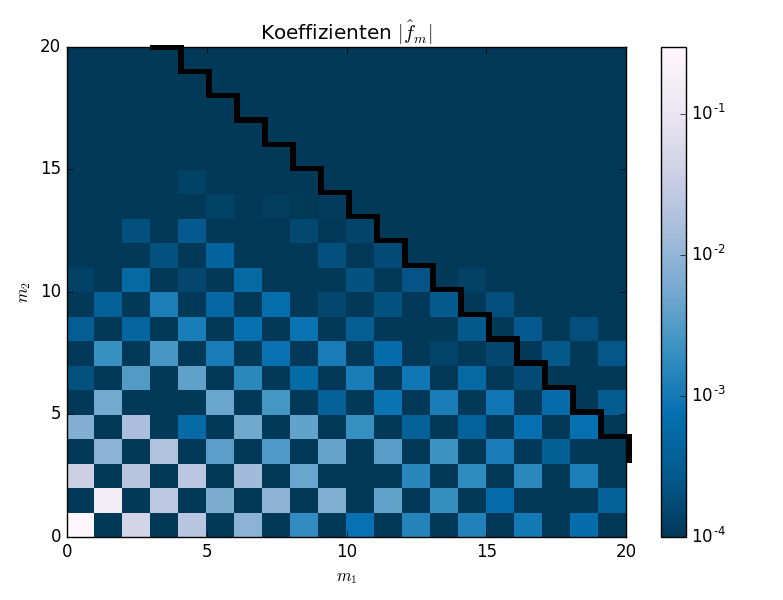
\includegraphics[width=\textwidth]{Figures/best_approx_coeffs_2d_example2log.png}
\caption{Koeffizienten $|\hat{f}_m|$ der Bestapproximation für $m_1,m_2=0,\dots,15$ der Funktion aus Beispiel \ref{bsp:bestapproxcoeffs2d}. Koeffizienten links unterhalb der schwarzen Linie erfüllen dabei $|m|\le 22$.}
\label{fig:bestapproxcoeffs2d}
\end{figure}
\end{mathbsp}

\section{Extraktion von Statistiken}
Gegeben sei die multivariate gPC-Approximation mit Summenschranke $P$ zu einer Funktion $f(Y)$ und einem Zufallsvektor $Y$ der Dimension $N$, also
\[f(Y)\approx f_M(Y)=\sum_{|m|\le P}\hat{f}_m\Phi_m(Y)\in\Poly_P^N,\quad m\in\N_0^N\]
Unter Ausnutzung der Orthogonalitätsbedingung (\ref{eqn:gpc_ortho_mv}) der Polynombasen lassen sich gewisse Statistiken der gPC-Approximation auf sehr einfache Art und Weise berechnen. Schlussendlich ist dies eine der größten Motivationen dafür, die Orthogonalbasis passend zur gegebenen Verteilung zu wählen.\\
Es ist $\gamma_{(0,\dots,0)}=1$, da für das nicht normalisierte Polynom $\Psi_0\equiv 1$ und eine Wahrscheinlichkeitsverteilung $F_Y$ gilt $\gamma_0=\E[\Psi_0^2(Y)]=\int 1\cdot 1dF_Y(y)=1$. Folglich gilt $\Phi_{(0,\dots,0)}(Y)= \frac{\Psi_0(Y)}{\sqrt{\gamma_0}}\equiv 1$ und für den Erwartungswert $\mu_f$
\begin{equation}
\label{eqn:gpc_approx_exp}
\begin{split}
\mu_f=\E[f(Y)]\approx \E[f_N(Y)]&=\int\left(\sum_{|m|\le P}\hat{f}_m\Phi_m(Y)\right)dF_Y(y)\\
&=\sum_{|m|\le P}\hat{f}_m\int\Phi_m(Y)dF_Y(y)\\
&=\sum_{|m|\le P}\hat{f}_m\E[\underbrace{\Phi_{(0,\dots,0)}(Y)}_{\equiv 1} \Phi_m(Y)]\\
&=\sum_{|m|\le P}\hat{f}_m\delta_{(0,\dots,0),m}=\hat{f}_{(0,\dots,0)}
\end{split}
\end{equation}
Die Varianz lässt sich dann berechnen als
\begin{align*}
\sigma^2_f=\text{var}(f(Y))&=\E[f^2(Y)]-\E[f(Y)]^2\\
&\approx \sum_{|m|\le P}\sum_{|n|\le P}\hat{f}_m\hat{f}_n\underbrace{\E[\Phi_m(Y)\Phi_n(Y)]}_{=\delta_{mn}}-\hat{f}_{(0,\dots,0)}^2\\
&=\sum_{0<|m|\le P}\hat{f}_m^2
\end{align*}
Die Standardabweichung ist folglich gegeben durch
\[\sigma_f=\sqrt{\text{var}(f(Y))}\approx\sqrt{\sum_{0<|m|\le P}\hat{f}_m^2}\]
Ist man an einer Approximation der Dichtefunktion von $f(Y)$ interessiert, so lässt sich diese mittels eines Histogramms und Samplings der Funktion $f_N(Y)=\sum_{|m|\le P}\hat{f}_m\Phi_m(Y)$ näherungsweise darstellen.\\[0.2cm]
Für höhere Momente gilt
\begin{align*}
\E[f^\ell(Y)]\approx \sum_{|m^{(1)}|,\dots,|m^{(\ell)}|\le P} \hat{f}_{m^{(1)}}\dots\hat{f}_{m^{(\ell)}}\underbrace{\E[\Phi_{m^{(1)}}(Y)\dots\Phi_{m^{(\ell)}}(Y)]}_{=\mathcal{T}_{m^{(1)},\dots m^{(\ell)}}}
\end{align*}
Diese Berechnung benötigt für $\ell>2$ eine einmalige Berechnung des Tensors $\mathcal{T}$. Dieser ist unabhängig von der betrachten Funktion $f$ und kann somit wieder verwendet werden.
\begin{mathbsp}
Für $N=1$ und $\ell=3$ ist der Momententensor $\mathcal{T}$ für $Y\sim \mathcal{N}(0,1)$ und zugehöriger orthonormaler Polynombasis $H_m$ der Hermite-Polynome für $P=2$ gegeben durch
\[\mathcal{T}=
\begin{tikzpicture}[every node/.style={anchor=north east,fill=white,minimum width=0.7cm,minimum height=7mm}]
\matrix (mA) [draw,matrix of math nodes]
{
0 & 0 & 1 \\
0 & \sqrt{2} & 0 \\
1 & 0 & 2\sqrt{2} \\
};

\matrix (mB) [draw,matrix of math nodes] at ($(mA.south west)+(0.2,1.5)$)
{
0 & 1 & 0 \\
1 & 0 & \sqrt{2} \\
0 & \sqrt{2} & 0 \\
};

\matrix (mC) [draw,matrix of math nodes] at ($(mB.south west)+(0.2,1.5)$)
{
 1 & 0 & 0 \\
 0 & 1 & 0 \\
 0 & 0 & 1 \\
};

\draw[dashed](mA.north east)--(mC.north east);
\draw[dashed](mA.north west)--(mC.north west);
\draw[dashed](mA.south east)--(mC.south east);
\end{tikzpicture}
\]
\end{mathbsp}